\chapter{Анализ данных топографических карт}
\label{ch:chap2}
Программа осуществляет чтение набора временных срезов топографических карт, соответствующих различным каналам ЭЭГ. Затем карты проходят предварительную обработку, включая обрезку и преобразование в черно-белый формат. На следующем этапе выполняется пороговая обработка изображений, что позволяет создать бинарную маску, отображающую активные и неактивные области.

На заключительном этапе временные срезы объединяются в видеоролик, предназначенный для последующего анализа. Также рассчитывается процент площади наименее активных зон для заданного канала, что позволяет оценить пространственно-временные характеристики минимальной активности мозга.
\section{Предобработка}

    \begin{enumerate}
        \item Загрузка данных
        \begin{enumerate}
            \item Чтение всех ранее созданных PNG-файлов в указанной директории
        \end{enumerate}
        \item Графическая обработка PNG-файлов с топографическими картами
        \begin{enumerate}
            \item Преобразование изображений в черно-белый формат по следующей формуле:
                \begin{equation}
                    I_{\text{gray}} = 0.299 \cdot R + 0.587 \cdot G + 0.114 \cdot B,
                    \label{eq:grayscale_conversion}
                \end{equation}
                    
                где:
                \begin{itemize}
                    \item \( I_{\text{gray}} \) — яркость пикселя в градациях серого,
                    \item \( R \) — значение красного канала (Red),
                    \item \( G \) — значение зелёного канала (Green),
                    \item \( B \) — значение синего канала (Blue),
                    \item \( 0.299 \), \( 0.587 \), \( 0.114 \) — веса цветовых каналов, основанные на их вкладe в яркость в соответствии с человеческим восприятием.
                \end{itemize}
            \item Обрезание изображения оптимизации последующей обработки
            \item Применение пороговой фильтрации для изображений по следующей формуле:
                \begin{equation}
                    I_{\text{binary}}(x, y) =
                    \begin{cases} 
                        I_{\text{max}}, & \text{если } I_{\text{input}}(x, y) > T, \\
                        I_{\text{min}}, & \text{иначе,}
                    \end{cases}
                    \label{eq:thresholding}
                \end{equation}

                где:
                \begin{itemize}
                    \item \( I_{\text{binary}}(x, y) \) — значение интенсивности пикселя в двоичном изображении,
                    \item \( I_{\text{input}}(x, y) \) — значение интенсивности пикселя в исходном изображении,
                    \item \( T \) — пороговое значение (\(T = 235\)),
                    \item \( I_{\text{max}} \) — максимальное значение интенсивности (например, \(255\) для 8-битных изображений),
                    \item \( I_{\text{min}} \) — минимальное значение интенсивности (например, \(0\) для 8-битных изображений).
                \end{itemize}
        \end{enumerate}
    \end{enumerate}
    В результате этапа предобработки формируется бинарное изображение топографической карты, на котором зоны с минимальной активностью головного мозга визуализированы в виде выделенных белым цветом областей.
Примеры временных срезов топографических карт для соответствующих каналов: \newline
\begin{figure}[!ht]
    \centering
    \begin{tabular}{cc}
        \begin{subfigure}[c]{0.3\textwidth}
            \centering
            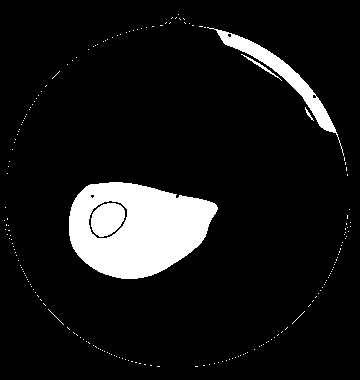
\includegraphics{images/topomap_delta_binary.png}
            \caption{}
        \end{subfigure}
        &
        \begin{subfigure}[c]{0.3\textwidth}
            \centering
            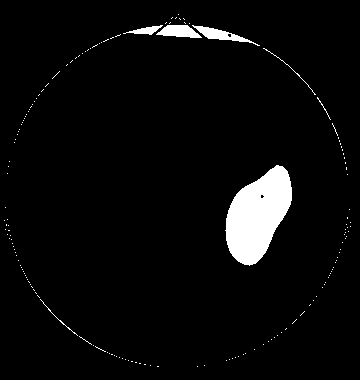
\includegraphics{images/topomap_theta_binary.png}
            \caption{}
        \end{subfigure}
    \end{tabular}
    \vspace{\abovecaptionskip}
    \begin{tabular}{ccc}
        \begin{subfigure}[c]{0.3\textwidth}
            \centering
            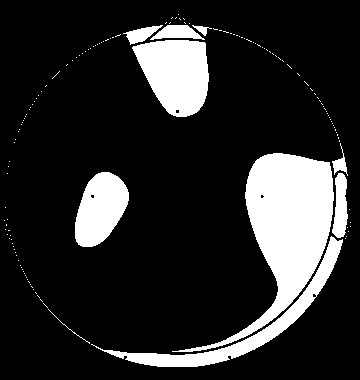
\includegraphics{images/topomap_alpha_binary.png}
            \caption{}
        \end{subfigure}
        &
        \begin{subfigure}[c]{0.3\textwidth}
            \centering
            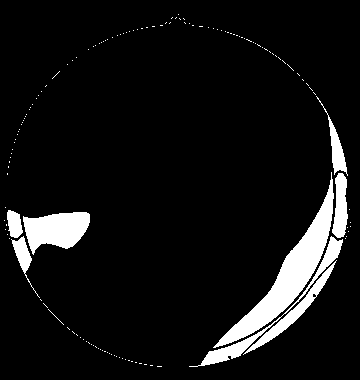
\includegraphics{images/topomap_beta_binary.png}
            \caption{}
        \end{subfigure}
        &
        \begin{subfigure}[c]{0.3\textwidth}
            \centering
            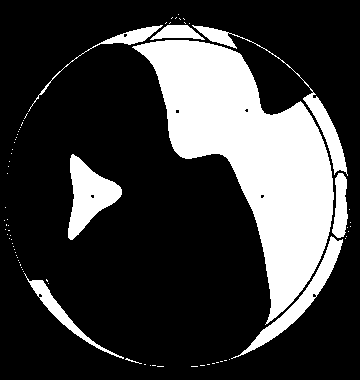
\includegraphics{images/topomap_gamma_binary.png}
            \caption{}
        \end{subfigure}
    \end{tabular}
    \caption{<Бинарные изображения топографических карт из \hyperref[fig:topomap_colored]{Рисунка \ref*{fig:topomap_colored}} построенные по соответствующим каналам. (а) - Delta-канал (0-4 Гц), (б) - Theta-канал (4-8 Гц), (в) - Alpha-канал (8-12 Гц), (г) - Beta-канал (12-30 Гц), (д) - Gamma-канал (30-45 Гц),}
    \label{fig:topomap_binary}
\end{figure}
    
\section{Создание видеоролика}
На данном этапе все сформированные бинарные представления топографических карт последовательно объединяются в видеоролик. Этот процесс позволяет представить динамическое изменение активности головного мозга в удобной визуальной форме, что упрощает анализ временных паттернов и пространственного распределения активности. Использование видеоформата способствует более наглядной интерпретации данных, позволяет отслеживать изменения в различных зонах мозга и улучшает эффективность последующего анализа.

\section{Вычисление неактивной области по временным интервалам}
В рамках обработки данных выполняется расчет доли неактивной области относительно общей площади топографической карты. Этот показатель выражается в процентах и позволяет количественно оценить распределение зон минимальной активности на карте.

Теоретически, неактивные области определяются как регионы с амплитудой сигналов ниже заданного порогового значения, которое устанавливается в зависимости от целей исследования и характеристик данных.

Процесс вычисления основывается на бинарной маске изображения, где активные области представлены единицами, а неактивные — нулями. Соотношение суммарной площади неактивных пикселей к общей площади карты рассчитывается по формуле:

\begin{equation}
P_{\text{inactive}} = \frac{S_{\text{inactive}}}{S_{\text{total}}} \times 100\%,
\end{equation}

где:
\begin{itemize}
    \item \( P_{\text{inactive}} \) — процент неактивной области,
    \item \( S_{\text{inactive}} \) — площадь неактивной области, определяемая как количество пикселей, соответствующих значениям ниже установленного порога,
    \item \( S_{\text{total}} \) — общая площадь топографической карты, выраженная в количестве всех пикселей.
\end{itemize}

Процентное выражение позволяет проводить сравнение между разными временными срезами или картами, что важно для выявления динамических изменений активности мозга.

\endinput